\chapter{Optimization Algorithm}
\label{chapter:optimization}

An optimization problem is any problem where a function $f:X \rightarrow Y$ is given, and we search for the point $x \in X$ such that $f(x)$ is minimal or maximal. Obviously the minimum or maximum must not exist, as the example $f: (0, 1) \rightarrow \mathbb{R}, x \mapsto x$ demonstrates by not having either. Investigating conditions on $X$, $Y$ and $f$ such that a minimum or maximum exists is mathematically interesting. However, when implementing an optimization algorithm the true minimum or maximum can sometimes not be found even if it exists and is instead replaced by a sufficiently good approximation.

First we want to first think about some variations of the problem.

In the case of a problem with additional conditions $P$ the minimum or maximum must satisfy we can consider at the subset $M:= \{x \in X: P(x)\} \subseteq X$. By finding the minimum or maximum of $f: M \rightarrow Y$ the problem is solved. Once again such a minimum or maximum must not exist, even if we have that one is present in $X$.


In the example dealt with in this work we are given some data points $((x_k, y_k))_{k \in \{1, 2, ..., n\}}$ and want to find a close approximation in the form of a function $g(x, a_1, a_2, ..., a_m)$ where for every $a = (a_1, ..., a_m)$ we have a function $g_a(x) : \mathbb{R} \rightarrow \mathbb{R}, x \mapsto g(x, a_1, ..., a_m)$. Searching for a good approximation can be reformulated as searching for the minimum of $r(a) := \sum_{k=1}^{n} |g_a(x_k) - b_k|^2$ or any other error function. This form of problem is called the Least Square Problem.

\subsection{Gradient Descent}

An iterative algorithm for finding the minimum of a differentiable function $f: \mathbb{R}^n \rightarrow \mathbb{R}$ is gradient descent. As the name suggests it uses information of the gradient $\nabla f$. Locally the negative gradient always points into the direction of greatest descent. The pseudocode of this approach is given below.

\begin{algorithm}[H] \label{alg:gradient_descent}
	\SetAlgoLined
	\DontPrintSemicolon
	\LinesNumbered
	\SetKwInOut{Input}{input}
	\SetKwInOut{Output}{output}
	\caption{Gradient Descent}
	
	\Input{$f: \mathbb{R}^n \rightarrow \mathbb{R}$ ... differentiable, $x_0 \in \mathbb{R}^n$}
	\Output{$x \in \mathbb{R}^n$}
	\BlankLine
	\Begin{
		\For{$n=0$ \KwTo max\_iterations}{
			\If{improvement is smaller than threshold}{
				break\;
			}
			set or calculate step size $\gamma_n$\;
			$x_{n+1} = x_n - \gamma_n \nabla f(x_n)$\;
		}
		$x = x_n$\;
	}
\end{algorithm}

If we consider a function with a local but not global minimum gradient descent might not converge to the optimum. An example of such a function can be seen in figure~\ref{fig:grad_descent_global_min_not_found} along with the first steps of gradient descent.

\begin{figure}[h]
	\centering
	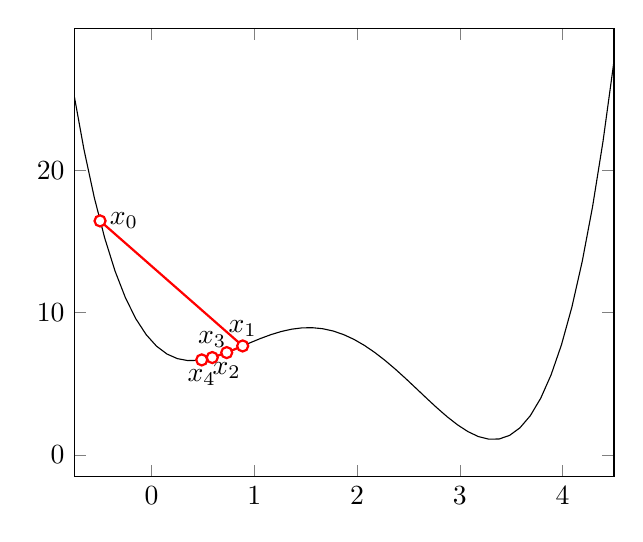
\begin{tikzpicture}
		\begin{axis}[xmin=-0.75, xmax=4.5, samples=100]
			\addplot[black] (x,x*x*x*x - 7*x*x*x + 14*x*x - 8*x + 8);
			\addplot[color=red,solid,thick,mark=*, mark options={fill=white}] 
			coordinates {
				(-0.5, 16.4375)
				(0.8875, 7.65428)
				(0.73223, 7.18773)
				(0.591558, 6.84009)
				(0.4894125, 6.67483)
			}; 
			\node [right] at (axis cs:  -0.5,  16.4375) {$x_0$};
			\node [above] at (axis cs:  0.8875, 7.65428) {$x_1$};
			\node [below] at (axis cs:  0.73223, 7.18773) {$x_2$};
			\node [above] at (axis cs:  0.591558, 6.84009) {$x_3$};
			\node [below] at (axis cs:  0.4894125, 6.67483) {$x_4$};
		\end{axis}
	\end{tikzpicture}
	\caption{The function has two local minimums. For this starting value and step size gradient descent approaches the local, but not global minimum.}
	\label{fig:grad_descent_global_min_not_found}
\end{figure}

Improvements can be made by choosing good step sizes, starting value or by starting with different values and comparing the results.

\section{Least Square Problem Algorithms}

% https://docs.scipy.org/doc/scipy/reference/generated/scipy.optimize.least_squares.html

Formally we are given a residual function $r_f(x)$ which tells us whether a function $f$ is a good approximation at the point $x$. We therefore want to find a way to minimize $||r(x)||^2$.

\subsection{Gauss–Newton Algorithm}

For linear functions it is easy to find the intersection with zero. If we linearize $r(x)$ locally we can approximate the intersection with zero by finding it of the linear approximating function.

\begin{figure}[h]
	\centering
	\begin{tikzpicture}
		\begin{axis}[xmin=0, xmax=5, samples=100]
			\addplot[black] (x,-x*x + 7);
			\addplot[red] (x,-2*x+8);
			\addplot[black] (x,0);
			\addplot[color=black,only marks,mark=*, mark options={fill=white}] 
			coordinates {
				(1, 6)
				(4, 0)
			};
		\end{axis}
	\end{tikzpicture}
	\caption{By approximating the black function by a line an approximation of the root has been found.}
	\label{fig:TODO}
\end{figure}

Iterating the linear approximating gives us the Gauss-Newton Method. By using Taylor's theorem we get the linear approximation $r(x) = r(a) + Dr(a)(x-a) + h(x)(x-a) \approx r(a) + Dr(a)(x-a)$ with $\lim\limits_{x\rightarrow a}h(x) = 0$. Rewriting this as $r(x) \approx Ax - b$ where $A := Dr(a)$ and $b := Dr(a)a-r(a)$ gives us the algorithm for this method.

\begin{algorithm}[H] \label{alg:gauss_newton}
	\SetAlgoLined
	\DontPrintSemicolon
	\LinesNumbered
	\SetKwInOut{Input}{input}
	\SetKwInOut{Output}{output}
	\caption{Gauss-Newton}
	
	\Input{$r: \mathbb{R}^n \rightarrow \mathbb{R}^m$ ... differentiable, $x_0 \in \mathbb{R}^n$}
	\Output{$x \in \mathbb{R}^n$}
	\BlankLine
	\Begin{
		\For{$n=0$ \KwTo max\_iterations}{
			\If{$x_n$ close enough to zero}{
				break\;
			}
			Calculate $A := Dr(x_n)$\;
			Calculate $b := A(x_n) - r(x_n)$\;
			Solve $A(x_{n+1}) = b$\;
		}
		$x = x_n$\;
	}
\end{algorithm}

Gauss-Newton is guaranteed to find a local minimum $x$ if $r$ is twice continuously differentiable in an open convex set including $x$, $Dr$ has a full rank and the initial value is close enough to $x$.

\subsection{Levenberg-Marquardt Algorithm}

\subsection{Trust Region Reflective Algorithm}
% https://www.applied-mathematics.net/LMvsTR/LMvsTR.pdf

% https://johnwlambert.github.io/gauss-newton/

\subsection{Dogleg Algorithm with Rectangular Trust Regions}